\chapter{GSAS-II Utility Computation Tools}\label{Chap:Utilities}

\section{Absorb: Compute X-ray Absorption Coefficient}\label{ref:Absorb}\index{program Absorb}

GSAS-II includes a program for computing the absorption of a material. It was originally created as a free-standing program that was also implemented as a web utility,
\footnote{A web calculator for x-ray absorption based on program Absorb is found at URL  https://11bm.xray.aps.anl.gov/absorb/}
but now is  accessed from inside the GSAS-II GUI. To access it, use the Calculate/"Run Absorb" menu command. This will open a window, as shown in Fig. \ref{fig:absorb1}. The next step in use is to add the elements that will be used in the computation. Use the Absorb/"New Element" menu command, to add the elements that will be needed. After the command is entered, a periodic table is shown, as seen in Fig. \ref{fig:absorb2}. Click on one or more elements in the table; note the color of the selected elements change as selected. Click on OK to close the periodic table window and return to the previous window for the Absorb program, which now lists computation results, but you will likely need to edit the chemical formula which is done by typing a number in the box to the right of the element and \textit{then pressing Enter}. 

\begin{figure}
    \centering
    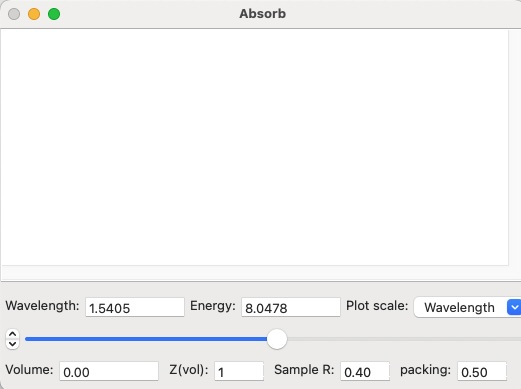
\includegraphics[width=0.5\linewidth]{figures/absorb1.jpg}
    \caption{Program Absorb: initial empty window}
    \label{fig:absorb1}
\end{figure}

\begin{figure}
    \centering
    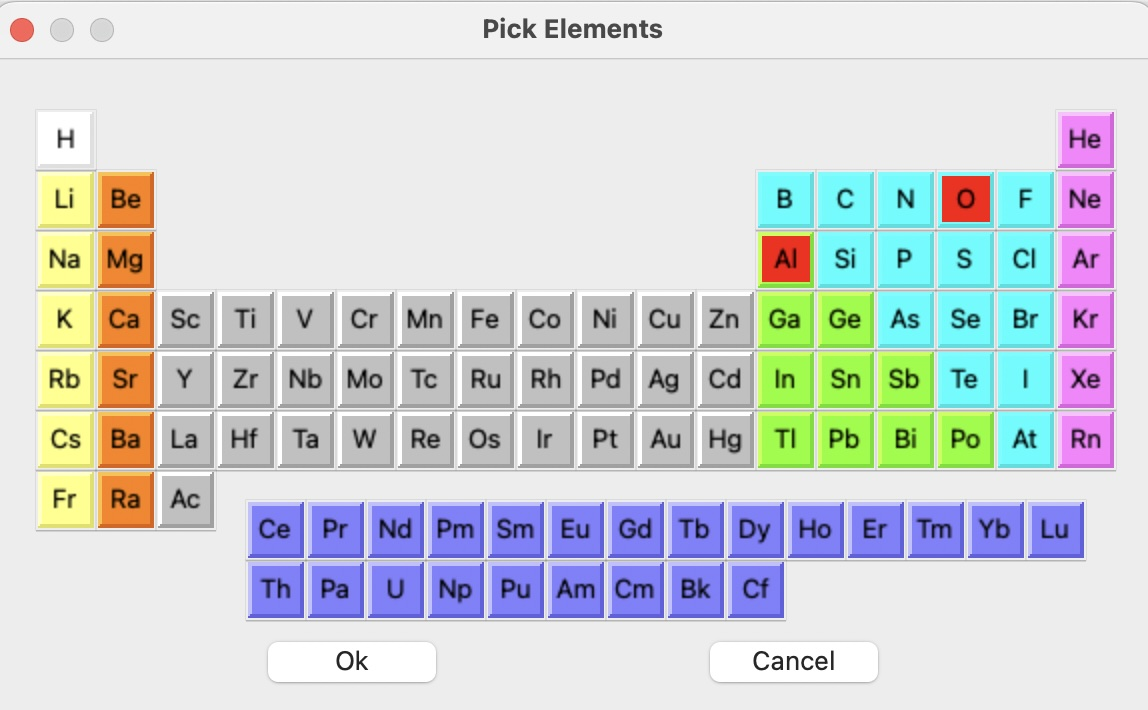
\includegraphics[width=0.5\linewidth]{figures/absorb2.jpg}
    \caption{Program Absorb: element selection}
    \label{fig:absorb2}
\end{figure}
Other input that you will likely supply includes the x-ray wavelength (or energy) and the sample radius (labeled as "Sample R") \textit{in mm}. Note that capillary dimensions are normally supplied as a diameter, so make sure you divide that by 2. The packing fraction (labeled here as "packing") is probably in the range of 0.4 to 0.6, so 0.5 is probably a good number. The "Volume" and "Z" values are used to estimate the crystallographic density, listed in the computations as the "Est. density". What is listed as the "powder density" is the crystallographic density multiplied by the packing fraction; this is the density used to compute x-ray absorption. The "Volume" and "Z" values likely do not need to be changed. Ideally, you will have measured the actual sample density, by weighing the sample and estimating the volume. If so, modify the packing fraction to get the powder density  to match what you measured. 

Note that the computations are not updated until you press "Enter" after changing any inputs. 
\begin{figure}
    \centering
    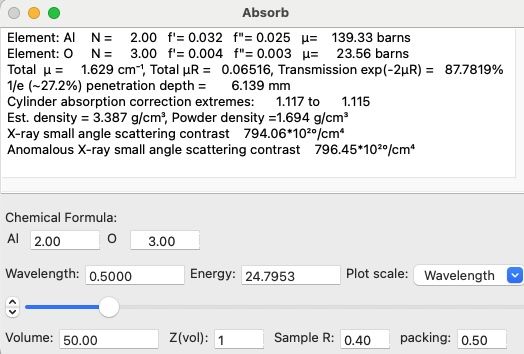
\includegraphics[width=0.5\linewidth]{figures/absorb3.jpg}
    \caption{Program Absorb: After element selection and stoichiometry editing}
    \label{fig:absorb3}
\end{figure}
The computed linear absorption coefficient value is reported as $\mu$ in cm${}^{-1}$, but for Debye-Scherrer geometry measurements, the key value is $\mu R$, as discussed in depth in section \ref{ref:muR}. Note the plots produced by program Absorb. The wavelength dependence plot will show if there are any absorption edges to be avoided and how much the wavelength will need to be changed to bring  $\mu R$ into the feasible range (red horizontal line) or recommended range (blue horizontal line). The correction vs. $2\theta$ plot shows how significant the correction will be over the data collection range. Note that this value is a measurement of transmission. A value of 20 indicates that only 95\% of the x-ray radiation is being lost to absorption. 

To confirm that a sample depth is thick enough for Bragg-Bretano measurements, you can also use program Absorb for that. Use the sample thickness divided by 2 as the radius. The transmission factor (listed after the $\mu R$ value) will represent the amount of x-ray radiation that would be transmitted through the sample at $2\theta$ of 180$^\circ$ and should be on the order of <5\% (noting that the path length increases by $1/cos\theta$ for $2\theta < 180^\circ$) as the actual losses will be lower.  

Use the Absorb/Quit menu command to exit the Absorb program. Exiting GSAS-II will also close Absorb.

\section{Fprime: Compute atomic scattering}\label{ref:Fprime}\index{program Fprime}

GSAS-II includes a program for computing the scattering factor curves for selected elements. It uses the same computation method as GSAS-II does for estimation of $f^\prime$ and $f^{\prime\prime}$ values, which are taken from a compilation made in 1981 by D. T. Cromer\index{Cromer, D.} and D. A. Liberman.\index{Liberman, D.}

absorption of a material. It was originally created as a free-standing program that was also implemented as a web utility,
\footnote{A web calculator for x-ray absorption based on program Absorb is found at URL  https://11bm.xray.aps.anl.gov/absorb/}
but now is  accessed from inside the GSAS-II GUI. To access it, use the Calculate/"Run Absorb" menu command. This will open a window, as shown in Fig. \ref{fig:absorb1}. The next step in use is to add the elements that will be used in the computation. Use the Absorb/"New Element" menu command, to add the elements that will be needed. After the command is entered, a periodic table is shown, as seen in Fig. \ref{fig:absorb2}. Click on one or more elements in the table; note the color of the selected elements change as selected. Click on OK to close the periodic table window and return to the previous window for the Absorb program, which now lists computation results, but you will likely need to edit the chemical formula which is done by typing a number in the box to the right of the element and \textit{then pressing Enter}. 


(section not started: \ref{needs more work})

\section{PlotXNFF: Plot form factors and scattering lengths}\label{ref:PlotXNFF}

(section not started: \ref{needs more work})